\begin{figure}[t]
\centering
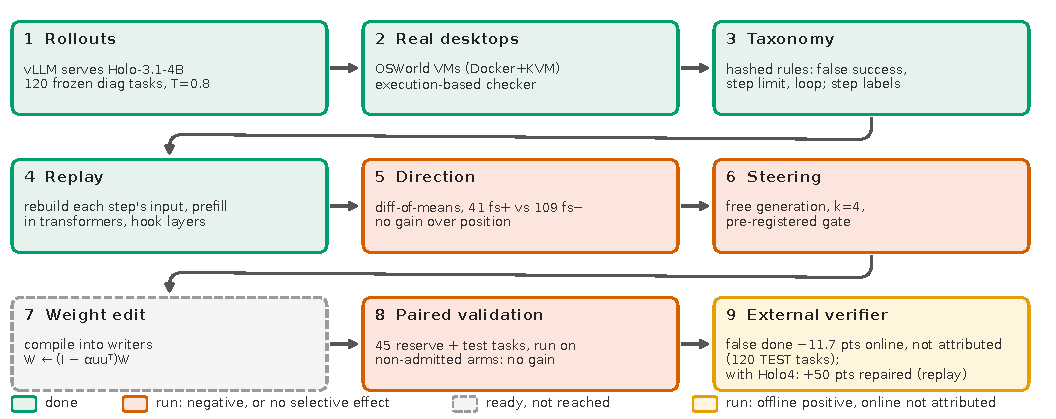
\includegraphics[width=\linewidth]{figs/pipeline.pdf}
\caption{\textbf{The pipeline and where it stands.} Stages 1--4 are complete and verified. The official direction analysis (5), on \bAdmFsPos{} admissible \fsp{} steps, finds no signal beyond position. Steering (6) has been run, and no candidate passes the gate. The compiled weight edit (7) is built and tested on null patches, but not reached because no candidate has been admitted. The paired online validation (8) was run anyway, on arms that had not been admitted (\S\ref{sec:online}), and shows no gain beyond the run-to-run noise of the original. An external verifier (9, \S\ref{sec:guard}) separates false from true successes offline; online, on the \OgN{} \textsc{test} tasks, the guarded run had fewer false ``done'' (\OgFdDiff{} points) with no measurable score change, but most of that drop came from episodes in which the guard never ran, so it is not attributed to the guard; handing its refusals to Holo4-27B adds \rbPrimDiff{} points of repairs (95\% CI \rbPrimDiffCi, \rbPrimEpisodes{} episodes), measured in replay only.}
\label{fig:pipeline}
\end{figure}
